
\chapter{Certified Programming}
\label{chap:certprog}

The Alba programming languages makes certain guarantees.
\begin{enumerate}
\item A program cannot crash.

\item There are not endless loops (i.e. the program cannot not freeze).

\item All functions perform according to their specification.
\end{enumerate}

The first point is achieved by a strict typing, a strict handling of pattern
match (all cases must be handled) and the lack of an undisciplined exception
processing. An undisciplined exception processing would be to allow the
throwing of exceptions without enforcement of the handling of exceptional
conditions.

The second point (no endless loops) is achieved by basing all recursions on
some argument which is decreased at each recursive call. This guarantees that
all functions must terminate.

The third point is achieved by implementing the curry howard isomorphism in
the form of propositions as types. It is possible to encode propositions like
$i > 0$ as a type and writing functions which return an inhabitant of these
types i.e. functions which generate a proof of the proposition.

Having this tool, it is possible to state some properties of functions and
prove these properties by writing functions which return proofs of the
desired properties.

In Alba a proof is just a functional programm. A proof of the implication $a
\imp b$ is a function which maps a proof of the proposition $a$ into a proof
of the proposition $b$.

Proofs in Alba are normal objects with the difference that these proof objects
do not exist at runtime. But they are data, which can be arguments to
functions. The functions can iterate over the proof data and can generate
other proof objects.

The purpose of this chapter is to demonstrate the possibility in Alba to write
functions and prove properties about these functions in the same language.




\newpage
\section{Logic}
\label{sec:certprog-logic}


In this chapter we use functional programming to prove some basic laws of
logic. The Alba compiler \emph{knows} how to handle propositions and is able
to do all the proofs in this chapter automatically. You are never required to
produce such proofs by hand.

But is very instructive to see how proofs of these basic laws of logic can be
generated by using functional programming. Therefore we give manual proofs
here.



\subsection{Ex Falso}

\emph{Ex falso quodlibet} i.e. from a false (or contradictory) assumption you
can conclude anything, is a basic law of logic. It is possible to prove this
law in Alba by writing a function with the signature

\begin{alba}
  ex_falso (pf: false) (A: Any): A :=
    ...
\end{alba}
%
The signature of this function gives the promise: \emph{Give me a proof of
  \code{false} and an arbitrary type and I return you an object of that
  type}. Since \code{a:Proposition} implies \code{a:Any} in Alba, all
propositions can be entered as actual arguments for \code{A}.


Remember that \code{false} is an inductive type with the following definition.
\begin{alba}
  class false: Proposition create
    -- no constructors
\end{alba}
%
Since there are no constructors we can complete the desired function

\begin{alba}
  ex_falso (pf: false) (A: Any): A :=
    inspect pf case
      -- empty pattern match, because there are no constructors
\end{alba}
%
Each case must return an object of the desired type. But since there are no
cases, there is nothing to be done.






\subsection{Negation}

Negation is defined in the prelude as
\begin{alba}
  (not) (a: Proposition): Proposition :=
    a => false
\end{alba}

We want to prove the contrapositive law of logic which states
\begin{alba}
  (a => b) => (not b => not a)
\end{alba}
for all propositions \code{a} and \code{b}. A proof of that fact would be
written in Alba as the function
%
\begin{alba}
  contrapositive a b (ab: a => b) (nb: not b): not a :=
    _      -- '_' means: Compiler, please generate a proof of 'not a'!
\end{alba}
%
It is not necessary to write such a proof by hand, because the compiler can
generate such a proof automatically. But if you want to write the proof
explicitly it looks like

\begin{alba}
  contrapositive a b (ab: a => b) (nb: not b): not a :=
    \ pa :=
        explicit_arguments
          nb (ab pa)
\end{alba}

\noindent Explanation: A proof of \code{not a} is a function which maps a
proof of \code{a} into a proof of false. If we have a proof of \code{a} we can
use the argument \code{ab} which maps a proof of \code{a} into proof of
\code{b} and then use \code{nb} which maps a proof of \code{b} into a proof of
\code{false} which is the desired result.

Since proof arguments are implicit in Alba, we have to use the keyword
\code{explicit\_argmuments} to give them explicitly. This keyword does not
exist in the actual Alba language. It is used here just to remind you that
proof arguments are given explicitly instead of letting the compiler infer
them.


Note that in classical logic the two propositions
\begin{alba}
  a  =>  b

  not b => not a
\end{alba}
%
are equivalent. This is not the case in constructive logic on which Alba is
based. Suppose we wanted to prove
%
\begin{alba}
  (not b => not a) => a => b
\end{alba}
%
in Alba. In order to do this we need a function
\begin{alba}
  contra2 a b (p: not b => not a) (pa: a): b :=
     ...
\end{alba}
%
It is not difficult to see that there is no way to generate a proof of \code{b}
by using the arguments. The second argument of the function is atomic i.e. it
is not a function which can be applied. The first argument is a function whose
type we can expand to get
\begin{alba}
  p: (b => false) => a => false
\end{alba}
%
\code{p} is a function with two arguments. There is no way to supply the first
argument. Therefore we cannot use \code{p} and have no possibility to return
an expression of type \code{b}.


However there is a double negation correspondence between classical and
constructive logic. Whenever classical logic is able to prove \code{a},
constructive logic is capable to prove \code{not not a}. I.e. we should be
able to prove
\begin{alba}
  (not b => not a) => a => not not b
\end{alba}
and define a function with the signature
%
\begin{alba}
  contra3 a b (p: not b => not a) (pa: a): not not b :=
    ...
\end{alba}
%
Now we have more possibilities because we are no longer required to prove
\code{b} directly, but only to derive \code{false} from \code{not b}. This
opens the possibility to use the function \code{p}.
%
\begin{alba}
  contra3 a b (p: not b => not a) (pa: a): not not b :=
    \ (nb: not b): false :=
        explicit_arguments
          (p nb) a
\end{alba}



\subsection{Disjunction}

Logical disjunction is defined in the prelude as the inductive type
%
\begin{alba}
  class
    (or) (a b: Proposition): Proposition
  create
    left:  a => a or b
    right: b => a or b
\end{alba}
%
i.e. you can either use a proof of \code{a} or a proof of \code{b} to generate
a proof of \code{a or b}.

It is a basic law of logic that \code{a or b} and \code{b or a} are
equivalent, i.e. we should be able to prove
%
\begin{alba}
  a or b  =>  b or a
\end{alba}
%
We prove this fact by defining the corresponding function which pattern
matches on the construction of \code{a or b}
%
\begin{alba}
  swap_or a b (p: a or b): b or a :=
    explicit_arguments
      inspect
        p
      case
        left  _ _ pa := right b a pa
        right _ _ pb := left  b a pb
\end{alba}

The propositions \code{a} and \code{b} are parameters of the proposition
\code{a or b}. Since parameters are the same for all constructors, it is not
allowed to bind variables to them. Therefore the anonymous variables \code{\_}
in the pattern match expression. Normally the parameters of the constructors
are implicit, but we have decided to supply the explicitly for educational
purposes.

Another law of logic states
\begin{alba}
  a or b  =>  (a => c) => (b => c)  =>  c
\end{alba}
%
i.e. whenever we have a prove of \code{a or b} and are able to conclude
\code{c} from \code{a} and \code{c} from \code{b}, then we are able to
conclude \code{c}.

A function which proves this fact is easy to implement by pattern matching on
the construction of \code{a or b}.

\begin{alba}
  eliminate_or a b c (ab: a or b) (ac: a => c) (bc: b => c): c :=
    explicit_arguments
      inspect
        ab
      case
        left  _ _ pa :=
          ac pa
        right _ _ pb :=
          bc pb
\end{alba}


\subsection{Conjunction}

\begin{alba}
  class
    (and) (a b: Proposition): Proposition
  create
    conjunction: a => b => a and b
\end{alba}


\begin{alba}
  swap_and (a b: Proposition) (p:a and b): b and a :=
    explicit_arguments
      inspect
        p
      case
        conjunction _ _ pa pb := conjunction b a pb pa
\end{alba}


\begin{alba}
  eliminate1_and (a b: Propositon) (p: a and b): a :=
    inpect p case
      conjunction _ _ pa pb := pa
\end{alba}



\subsection{De Morgan's Laws}

The De Morgan's Laws are other basic laws of logic. The first of the De
Morgan's laws states the equivalence of the two statements
\begin{alba}
  not (a or b)

  not a and not b
\end{alba}
%
In order to prove the equivalence we have to prove both directions.
\begin{alba}
  de_morgan1_forward
    (a b: Proposition)
    (nab: not (a or b))
    : not a and not b :=
      explicit_arguments
        conjunction (not a) (not b) na nb where
          na: not a :=
             \ (pa: a): false :=
                nab (left a b pa)
          nv: not b :=
             \ (pb: a): false :=
                nab (right a b pb)
\end{alba}

\begin{alba}
  de_morgan1_backward
    (a b: Proposition)
    (nab: not a and not b))
    : not (a or b) :=
      explicit_arguments
        \ (a_or_b: a or b): false :=
          inspect nab case
            conjunction _ _ na nb :=
              inspect a_or_b case
                left _ _ pa :=
                   na pa
                right _ _ pb :=
                   nb pb
\end{alba}


There is a second De Morgan's law stating the equivalence of
\begin{alba}
  not a or not b

  not (a and b)
\end{alba}

The forward direction can be proved by the function
\begin{alba}
  de_morgan2_forward
    (a b: Proposition)
    (nab: not a or not b)
    : not (a and b) :=
      explicit_arguments
        \ (a_and_b: a and b): false :=
          inspect a_and_b case
            conjunction _ _ pa pb :=
              inspect nab case
                left _ _ na :=
                   na pa
                right _ _ nb :=
                   nb pb
\end{alba}


In trying to prove the backward direction we face some difficulties. In order
to prove \code{not a or not b} we have to prove either \code{not a} or
\code{not b}. The only premise we have is \code{not (a and b)} which is a
function mapping any proof of \code{a and b} into \code{false}.

This proof is not possible in constructive logic. Therefore it is not possible
to prove it in Alba either.

In order to prove a disjunction in constructive logic we have to decide which
of the two possibilities of \code{not a or not b} we want to prove. There is
no possibility to make such a decision by looking only at \code{not (a and
  b)}.





\subsection{Existential Quantification}

The existence of an object with a certain property is expressed in Alba by the
inductive type
%
\begin{alba}
  class
    exist A (f: Predicate A): Proposition
  create
    witness x: f x -> exist f
\end{alba}
%
i.e. the existence of an object with a certain property is proved by providing
a witness and a proof that the witness satisfies the required property.

In Alba we write
%
\begin{alba}
  some (x:A): f x

  -- or

  some x: f x   -- if the type 'A' can be inferred from the context
\end{alba}
%
as another way to express the proposition
%
\begin{alba}
  exist f
\end{alba}

A basic law of logic states
%
\begin{alba}
  (some x: f x) => (all x: f x => a) => a
\end{alba}
%
Proofs using this law reads like
\begin{quote}
  We know that there exists an object satisfying $f$. Let $x$ be such an
  object satisfying $f$. From $ f x$ we can conclude $a$. Therefore $a$ is
  valid.
\end{quote}

We can prove this law in Alba by writing the function
\begin{alba}
  exist_elim
    A (f: Predicate A) (ex: some x: f x)
    a (p: all x: f x => a): a :=
      explicit_arguments
        inspect ex case
          witness _ _ x pf :=
            p x pf
\end{alba}


Like for logical disjunction and conjunction there two De Morgan's laws for
existential and universal quantification. The first law states the equivalence
of
\begin{alba}
  not (some x: f x)

  all x: not (f x)
\end{alba}
or in words
\begin{quote}
  If there are no objects satisfying a certain property, then all objects do
  not satisfy the property. And if all objects do not satisfy a propert, then
  there are no objects satisfying the property.
\end{quote}

The proofs of the forward and backward direction are not complicated.

\begin{alba}
   ex_de_morgan1_forward
     A (f: Predicate A)
     (nex: not (some x: f x))
     : all x: not (f x) :=
       \ x (pf: f x): false :=
          nex (witness _ _ x pf)
\end{alba}


\begin{alba}
  ex_de_morgan1_backward
     A (f: Predicate A)
     (allnot: all x: not (f x))
     : not (some x: f x) :=
       \ (ex: some x: f x): false :=
          explicit_arguments
            inspect ex case
              witness _ _ x pf :=
                allnot x pf
\end{alba}

The second De Morgan's law states the equivalence of
\begin{alba}
  some x: not (f x)

  not all x: f x
\end{alba}

The forward direction is easy.

\begin{alba}
  ex_de_morgan2_forward
    A (f: Predicate A)
    (some_not: some x: not (f x))
    : not (all x: f x) :=
     explicit_arguments
       \ (pall: all x: f x): false :=
         inspect some_not case
           witness _ _ x nf :=
             nf (pall x)
\end{alba}

However the backward direction is not possible to prove. Constructive logic
requires us to find a witness in order to prove
\begin{alba}
  some x: not (f x)
\end{alba}
%
But the premise
%
\begin{alba}
  not all x: f x
\end{alba}
does not give us any possibility to extract a witness which does not satisfy
the property \code{f}



\subsection{Equality}

Equality is defined in Alba as an inductive type.
\begin{alba}
   class
     (=) (A: Any) (a:A): Predicate A
   create
     reflexive: a = a
\end{alba}

Note that the type \code{A} and the object \code{a} are parameters of the
inductive type. The expression \code{(a =)} is a predicate i.e. a function
\code{\textbackslash\ x := a = x} mapping each object \code{x} into the
proposition \code{a = x}.

In the proposition \code{a = b} the character of left argument \code{a} and
the right argument \code{b} is different. The first argument is a parameter
and the second argument is an index.

There is only one constructor to construct an equality proposition. The
constructed equality is that an object is equal to itself. In order to prove
\code{all (n:Natural): n + 0 = n} we need a function, mapping any natural
number \code{n} into a proof of \code{n + 0 = n}.

Equal objects need not be represented by identical syntactical expressions
because of the possibility of reduction.

Equality defined with the above inductive type is a rather strong
property. This kind of equality is also known as \emph{Leibniz equality} which
means that two equal objects satisfy the same properties.
%
\begin{alba}
  leibniz (A: Any) (a b:A) (eq: a = b) (f: Predicate A): f a => f b :=
    ...
\end{alba}


We can prove this theorem by a pattern match on the proof of the equality.
%
\begin{alba}
  leibniz (A: Any) (a b:A) (eq: a = b) (f: Predicate A): f a => f b :=
    inspect
      eq                                  -- inspected proof object
      (\ x (p: a = x): Proposition :=     -- elimination function
         f a => f x)
    case
      reflexive :=
        \ pa  := pa
\end{alba}
%
In order to see why the proof is correct we have added the elimination
function into the pattern match expression. The arguments of an elimination
function are the indices of the inductive type and an object of the inductive
type. The index of \code{a = b} is \code{b} and the object of the inductive
type is \code{eq}.

If we apply the elimination function to the two arguments
\code{b} and \code{eq}, we get the required result type \code{f a => f b} of
the pattern match expression. This shows that the elimination function is
correct.

Note that the only constructor \code{reflexive} constructs \code{a = a},
i.e. the index is \code{a}. Therefore the expression on the right side of the
case must construct an object of type \code{f a => f a}. The identity function
is a proof of this trivial implication.

In a similar manner we can prove the symmetry of the equality relation.

\begin{alba}
   equality_is_symmetric
     (A: Any) (a b: A) (eq: a = b): b = a :=
       inspect
         eq
         (\ x p := x = a)
       case
         reflexive := reflexive
\end{alba}

The proof of transitivity follows the same pattern.

\begin{alba}
   equality_is_transitive
     (A: Any) (a b: A) (ab: a = b): all c: b = c => a = c :=
       inspect
         ab
         (\ x p := all c: x = c => a = c)
       case
         reflexive :=
           \ c p := p
\end{alba}

The key of understanding the proof is to use the elimination function to
compute the required result on the right side of the constructor. By feeding
the index \code{b} and the proof object \code{ab} into the elimination
function we get the required proposition
%
\begin{alba}
  all c: a = c => a = c
\end{alba}
%
which is rather easy to prove.







\newpage
\section{Relations}
\label{sec:certprog-relations}


\subsection{Basic Properties}


In the following we consider endorelations i.e. binary relations where both
domains are the same. For endorelations we can define what it means to be
reflexive, transitive and symmetric.

\begin{alba}
  is_reflexive (A:Any) (r: Endorelation A): Proposition :=
    all a: r a a

  is_transitive (A:Any) (r: Endorelation A): Proposition :=
    all a b c: r a b => r b c => r a c

  is_symmetric (A:Any) (r: Endorelation A): Proposition :=
    all a b: r a b => r b a
\end{alba}



\subsubsection{Transitive Closure}

Next we define the transitive closure $r^+$ of a relation $r$. Graphically the
construction of $r^+$ from $r$ looks like.

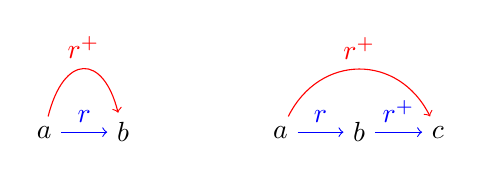
\begin{tikzpicture}
  \node (a0) at (0,0) {$a$};
  \node (b0) at (1,0) {$b$};

  \node (a) at (3,0) {$a$};
  \node (b) at (4,0) {$b$};
  \node (c) at (5,0) {$c$};

  \draw [->,blue] (a0) edge node[above]{$r$} (b0);
  \draw [->,red]
     (a0)
     .. controls (0.25,1) and (0.75,1)
     .. node[above] {$r^+$} (b0);

  \path[->,blue] (a) edge node[above] {$r$} (b);
  \path[->,blue] (b) edge node[above] {$r^+$}    (c);
  \draw[->,red]  (a) .. controls (3.5,1) and (4.5,1) ..  node[above] {$r^+$}  (c);
\end{tikzpicture}


In Alba we write

\begin{alba}
  class
    plus (A:Any) (r: Endorelation A): Endorelation A
      -- 'r.plus' is the transitive closure of 'r'
  create
    init a b:
      r a b
      => r.plus a b
    step a b c:
      r a b
      => r.plus b c
      => r.plus a c
\end{alba}

The definition uses an inductive type. It has two constructors. The
\code{init} constructor allows us to conclude $r^+ a b$ from $r a b$.  The
\code{step} constructor allows us to conclude $r^+ a c$ from $r a b$ and $r^+
b c$.

By intuition we see that the relation $r^+$ is transitive. But in
order to be sure we need a proof. In order to proof transitivity we have to
prove
%
$$
 r^+ a b \imp r^+ b c \imp r^+ a c
$$
%
for all $a$, $b$ and $c$
i.e. we need a function which looks like
%
\begin{alba}
  f a b c (pab: r.plus a b) (pbc: r.plus b c): r.plus a c :=
    ...
\end{alba}
%
We can do an induction proof on \code{pab: r.plus a b} which generates two
cases.

One case is that \code{r.plus a b} has been constructed
by \code{init a b rab}. In that case we can use the step constructor with
\code{ab: r a b} and \code{pbc: r.plus b c} to construct \code{r.plus a c}.

The second case is that  \code{r.plus a b} has been constructed by \code{step
  a x b (ax: r a x) (pxb: r.plus x b)}. Now we can use the induction
hypothesis to construct from \code{pxb} and \code{pbc} a proof of \code{r.plus
  x c} and then the step constructor to generate a proof of \code{r.plus a c}.


\begin{alba}
  plus_transitive A (r:Endorelation A): r.plus.is_transitive :=
    f a b c (pab: r.plus a b) (pbc: r.plus b c): r.plus a c :=
      inspect
        pab
      case
        init a b :=   -- implicit argument '_: r a b'
            -- a -> b +> c
          step a b c

        step a x b :=
            -- implicit arguments _:  r a x
            --                    _: r.plus x b
            {: goal: a -> x +> b +> c
               by a recursive call to f we prove x +> c
               and then use the step constructor to prove a +> c :}
          step a x c
          where
             _: r.plus x c := f x b c
\end{alba}



\subsubsection{Reflexive Transitive Closure}

In the same manner as the transitive closure we can define the reflexive
transitive closure of a relation.

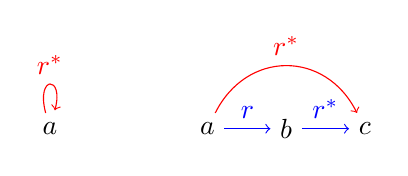
\begin{tikzpicture}
  \node (reflexive) at (0,0) {$a$};
  \node (a) at (2,0) {$a$};
  \node (b) at (3,0) {$b$};
  \node (c) at (4,0) {$c$};

  \path (reflexive) edge [loop above,red] node {$r^*$} (reflexive);

  \path[->,blue] (a) edge node[above] {$r$} (b);
  \path[->,blue] (b) edge node[above] {$r^*$}    (c);
  \draw[->,red]  (a) .. controls (2.5,1) and (3.5,1) ..  node[above] {$r^*$}  (c);
\end{tikzpicture}

\vbox{
\begin{alba}
  class
    star (A:Any) (r: Endorelation A): Endorelation A
      -- 'r.star' is the reflexive transitive closure of 'r'
  create
    init a:
      r.star a a

    step a b c:
      r a b
      => r.star b c
      => r.star a c
\end{alba}}

Having the definition we prove that the reflexive transitive closure is
transitive.

\begin{alba}
  star_transitive A (r:Endorelation A): r.star.is_transitive :=
    f a b c (sab: r.star a b) (sbc: r.star b c): r.star a c :=
      inspect
        sab
      case
        init a :=
          sbc  -- a = b in this case

        step a x b :=
          step a x c where
            hypo: r.star x c := f x b c
\end{alba}



\subsubsection{Equivalence Closure}

It is possible to convert any relation into an equivalence relation.

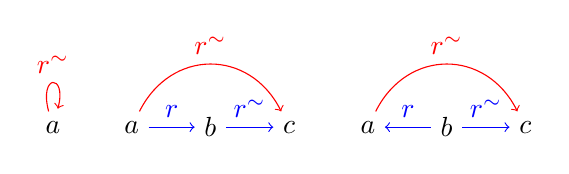
\begin{tikzpicture}
  \node (a0) at (0,0) {$a$};
  \path (a0) edge [loop above,red] node {$r^\sim$} (a0);

  \node (a1) at (1,0) {$a$};
  \node (b1) at (2,0) {$b$};
  \node (c1) at (3,0) {$c$};
  \draw[->,blue] (a1) edge node[above]{$r$} (b1);
  \draw[->,blue] (b1) edge node[above]{$r^\sim$} (c1);
  \draw[->,red] (a1) .. controls (1.5,1) and (2.5,1) .. node [above]{$r^\sim$} (c1);

  \node (a2) at (4,0) {$a$};
  \node (b2) at (5,0) {$b$};
  \node (c2) at (6,0) {$c$};
  \draw[<-,blue] (a2) edge node[above]{$r$} (b2);
  \draw[->,blue] (b2) edge node[above]{$r^\sim$} (c2);
  \draw[->,red]   (a2) .. controls (4.5,1) and (5.5,1) .. node [above]{$r^\sim$} (c2);
\end{tikzpicture}


\begin{alba}
  class
    equivalence A (r: Endorelation A): Endorelation A
  create
    init a:
     r.equivalence a a

    forward a b c:
      r a b => r.equivalence b c => r.equivalence a b

    backward a b c:
      r b a => r.equivalence b c => r.equivalence a b
\end{alba}


The equivalence closure is transitive.

\begin{alba}
  equivalence_is_transitive
    A (r: Endorelation A)
    : r.equivalence.is_transitive :=
    f a b c ab bc: r.equivalence a c :=
      inspect ab case
        forward a x b :=
          forward a x c where
            xc: r.equivalence x c := f x b c

        backward a x b :=
          backward a x c where
            xc: r.equivalence x c := f x b c
\end{alba}

The equivalence closure is symmetric.

\begin{alba}
  equivalence_is_symmetric
    A (r: Endorelation A)
    : r.equivalence.is_symmetric :=
    f a b ab: r.equivalence b a :=
      inspect ab case
        forward a x b :=   -- i.e. 'r a x' is valid
          equivalence_is_transitive r b x a where
            _: r.equivalence b x := f x b
            _: r.equivalence x a := backward x a a
            _: r.equivalence a a := init a

        backward a x b :=  -- i.e. 'r x a' is valid
          equivalence_is_transitive r b x a where
            _: r.equivalence b x := f x b
            _: r.equivalence x a := forward x a a
            _: r.equivalence a a := init a
\end{alba}






\subsection{Diamonds and Confluence}


A relation is a diamond if it is always possible to join two steps with a
single step.

\begin{alba}
  is_diamond A (r: Endorelation A): Proposition :=
      {:   a  ->  b
           |      |
           v      v
           c  -> some d :}
    all a b c:
      r a b
      => r a c
      => some d: r b d and r c d
\end{alba}


A relation is confluent if its reflexive transitive closure is a diamond.

\begin{alba}
  is_confluent A (r: Endorelation A): Proposition :=
    r.star.is_diamond
\end{alba}



We prove that a diamond relation is confluent. Before doing that, we prove a
stripe lemma.

\begin{alba}
  stripe_lemma
    A
    (r: Endorelation A)
    (rdia: r.is_diamond)
    : all a b c:                       --  a *> b
        r.star a b =>                  --  |    |
        r a c =>                       --  v    v
        some d: r b d                  --  c *> d?
                and
                r.star c d :=
     f a b c sab rac :=
       inspect sab case   -- a = b, therefore we use d = c as witness
         init a :=
           _: some d: r a d and r.star c d  where
             _: r.star c c := init c

         step a x b :=
           {:  a  -> x  *> b
               |     |     |
               v     v     v
               c  -> e? *> d? :}
           _ where
             exist_d: some d: r b d and r.star e d := f x b e
             exist_e: some e: r x e and r c e      := rdia a x c
\end{alba}

Then we can prove that a diamond relation is confluent.

\begin{alba}
  diamond_is_confluent
    A
    (r: Endorelation A)
    (rdia: r.is_diamond)
    : r.is_confluent
    :=
      f a b c sab sac: exist d: r.star b d and r.star c d :=
        inspect sab case
          init a :=            -- a = b, therefore we can use d = c
            _ where            --        as witness
              _: r.star b c := sac
              _: r.star c c := init c

          step a x b :=
            {:  a  ->  x  *>  b
                *      *      *
                v      v      v
                c  ->  e? *>  d? :}
            _ where
              exist_d: some d: r.star b d and r.star e d := f x b e
              exist_e: some e: r.star x e and r c e := stripe_lemma r a c x

\end{alba}




\newpage
\section{Lists}
\label{sec:certprog-lists}


In the following we use the definition of the list type from the prelude.

\begin{alba}
  class
    List (A:Any): Any
  create
    [] : List A
    (^): A -> List A -> List A
\end{alba}
%
Note that the operator $\caret$ is right associative and has the
highest precedence of all arithmetic operators.



\subsection{Concatenation}


A standard definition of list concatenation looks like

\begin{alba}
  (+) A (a b: List A): List A :=
    inspect a case
      [] :=
        b
      h ^ t :=
        h ^ (t + b)
\end{alba}
Note that the operator $+$ is left associative.


List concatenation is associative
%
\begin{alba}
  sum_associates A (a b c: List A): a + b + c = a + (b + c) :=
    inspect a case
      h ^ t :=
        goal where
          goal: h ^ t + b + c = h ^ t + (b + c) :=
            via
               h ^ t + b + c
               h ^ (t + b + c)      -- def (+)
               h ^ (t + (b + c))    -- hypo
               h ^ t + (b + c)      -- def (+)
          hypo: t + b + c = t + (b + c) :=
            sum_associates t b c
\end{alba}


\begin{alba}
  nil_right_neutral A (a: List A): a + [] = a :=
    inspect a case
      h ^ t :=
        goal where
          goal: h ^ t + [] = h ^ t :=
            via
              h ^ t + []
              h ^ (t + [])   -- def (+)
              h ^ t          -- hypo
          hypo: t + [] = t :=
            nil_right_neutral t
\end{alba}





\subsection{Reversal}



A simple function to reverse a list looks like

\begin{alba}
  reverse A (a: List A): List A :=
    inspect a case
      [] :=
        []
      h ^ t :=
        reverse t + [h]
\end{alba}


Next we prove a theorem which shows how reversal and concatenation
interact. Specifically we want to prove
\begin{alba}
  (a + b).reverse = b.reverse + a.reverse
\end{alba}

\begin{alba}
  reversal_of_concatenation
    A
    (a b: List A)
    : (a + b).reverse = b.reverse + a.reverse :=
      inspect a case
        h ^ t :=
          goal where
             goal: reverse (h ^ t + b) = reverse b + reverse (h ^ t) :=
               via
                 h ^ (t + b) |> reverse                     -- def '+'
                 h ^ (reverse b + reverse t) |> reverse     -- hypo
                 (b.reverse + t.reverse) + [h]              -- def 'reverse'
                 b.reverse + (t.reverse + [h])              -- '+' assoc
                 b.reverse + (h ^ t).reverse                -- def 'reverse'

             hypo: (t + b).reverse = b.reverse + t.reverse :=
               reversal_of_concatenation t b
\end{alba}


It is intuitively clear, that a double reversal of a list results in the
original list. We prove this property by
%
\begin{alba}
  double_reversal A (a: List A): a.reverse.reverse = a :=
    inspect a case
      h ^ t :=
        goal where
          goal: (h ^ t).reverse.reverse = h ^ t :=
            via
              (t.reverse + [h]).reverse
              [h].reverse + t.reverse.reverse
              [h] + t
          hypo: t.reverse.reverse = t :=
            double_reversal t
\end{alba}



\subsection{Tail Recursion}

Neither concatenation nor reversal are tail recursive. Furthermore definition
of list reversal is rather inefficient because of the $n^2$
complexity. However we can find equivalent functions which are tail recursive
and efficient.

We need an auxiliary function which reverses a list and prepends it in front
of another list.

\begin{alba}
  reverse_prepend A (a b: List A): List A :=
      -- prepend the reversal of 'a' in front of 'b'
    inspect
      a
    case
      [] :=
        b
      h ^ t :=
        t.reverse_prepend (h ^ b)
\end{alba}


We prove that the function does exactly what we are expecting it to do.

\begin{alba}
  reverse_prepend_correct
    A (a b: List A)
    : a.reverse_prepend b = a.reverse + b :=
      inspect a case
        h ^ t :=
          goal where
            goal: (h ^ t).reverse_prepend  b = (h ^ t).reverse + b :=
              via
                t.reverse_prepend (h ^ b)            -- def
                t.reverse + h ^ b                    -- hypo
                t.reverse + ([h] + b)                -- def '+'
                t.reverse + [h] + b                  -- assoc '+'
                (h ^ t).reverse + b                  -- def 'reverse'
             hypo: t.reverse_prepend (h ^ b) = t.reverse + h ^ b :=
               reverse_prepend_correct t (h ^ b)
\end{alba}


It is obvious that
%
\begin{alba}
  a.reverse_prepend [] = a.reverse
\end{alba}
%
is valid which is a direct consequence of the previous theorem. Alba allows to
override a function definition by an equivalent definition. Therefore we can
substitute the inefficient, non-tail-recursive definition of \code{reverse} by
a more efficient and tail recursive version.

\begin{alba}
  reverse A (a: List A): List A :=
    a.reverse_prepend []
\end{alba}

The definition of list concatenation is efficient, but not tail recursive. By
using the proved theorems we see the following equivalence
%
\begin{alba}
  a + b   =  a.reverse.reverse + b
          =  a.reverse.reverse_prepend b
\end{alba}

Using this, we are able to override the definition of list concatenation by a
tail recursive one

\begin{alba}
  (+) A (a b: List A): List A :=
    a.reverse.reverse_prepend b
\end{alba}

Overriding a definition has no effect during compilation. The original
definition remains to analyze properties. However as soon as the compiler
generates executable code, it replaces the original definition by the
definition which overrides the original definition. It is just an optimization
of the runtime.





\subsection{Specified Types}

In the previous section we defined a function \code{reverse\_prepend} which
should reverse a list and prepend it in front of another list. In a second
step we proved that the function does the expected.

This signals that we might be able to use a specified type (i.e. a type whose
inhabitants satisfy a specification) as a result and implement the function
and the proof of its specification hand in hand.

A specified type is an inductive type of the form
%
\begin{alba}
   class Specified A (f: Predicate A): Any create
     specified x: f x -> Specified f
\end{alba}

The type \code{Specified} is known to the compiler and instead of writing
%
\begin{alba}
  Specified (\ (x:T) := exp)
\end{alba}
%
we can use syntactic sugar and write
%
\begin{alba}
  {x: T : exp}
  -- or
  {x: exp}     -- if the type 'T' can be inferred from the context.
\end{alba}


If we use a specified type in \code{reverse\_prepend} we get the signature
\begin{alba}
  reverse_prepend A (a b: List A): {c: c = a.reverse + b} :=
    ...
\end{alba}

Any implementation of \code{reverse\_prepend} must satisfy the specification
i.e. it has to return a list \code{c} which satisfies
\begin{alba}
  c = a.reverse + b
\end{alba}


The implementation of the function includes the proof of the specification.

\begin{alba}
  reverse_prepend A (a b: List A): {c: c = a.reverse + b} :=
    inspect a case
      [] :=
        specified b where
          _: b = [].reverse + b := _

      h ^ t :=
        inspect t.reverse_prepend (h ^ b) case
          specified c :=
            specified c where
              _: c = (h ^ t).reverse + b :=
                via t.reverse + (h ^ b)      -- hypo
                    t.reverse + ([h] + b)    -- def '+'
                    t.reverse + [h] + b      -- '+' assoc
                    (h ^ t).reverse + b      -- def 'reverse'
\end{alba}


Since the Alba compiler \emph{knows} the mechanics of a specified type, we can
omit one pattern match.

\begin{alba}
  reverse_prepend A (a b: List A): {c: c = a.reverse + b} :=
    inspect a case
      [] :=
        specified b

      h ^ t :=
        t.reverse_prepend (h ^ b) where
          _ c (p: c = t.reverse + (h ^ b))
            : c = (h ^ t).reverse + b :=
             via t.reverse + (h ^ b)      -- 'p'
                 t.reverse + ([h] + b)    -- def '+'
                 t.reverse + [h] + b      -- '+' assoc
                 (h ^ t).reverse + b      -- def 'reverse'
\end{alba}

In this definition we give the compiler a hint on how to transform a proof of
the specification of the recursive call into a proof of the specification of
the outer call.

In the runtime all specifications and proofs are erased. Therefore the
definition of the function \code{reverse\_prepend} in this chapter and the
previous chapter are identical in the runtime.








\section{Natural Numbers}


The type of natural numbers is defined in the prelude inductively.

\begin{alba}
  class Natural create
    0: Natural
    successor: Natural -> Natural
\end{alba}

The number $1$ is the constant

\begin{alba}
  1: Natural := 0.successor
\end{alba}

The compiler \emph{knows} of this type and implements it as a efficient
segmented array to represent arbitrary precision arithmetic. Furthermore all
arithmetic functions like addition, multiplication and relational operators
are implemented as efficient functions. But all these builtin functions behave
as the following functions defined recursively on the inductive type above.





\subsection{Arithmetic}


\subsubsection{Addition}


First we need addition
\begin{alba}
  (+) (a b: Natural): Natural :=
    inspect a case
      0 :=
        b
      n.successor :=
        (n + b).successor
\end{alba}


Addition is associative
%
\begin{alba}
  plus_is_associative (a b c: Natural): a + b + c = a + (b + c) :=
    inspect a case
      n.successor :=
        via
          n.successor + b + c
          (n + b + c).successor
          (n + (b + c)).successor
          n.successor + (b + c)
        where
          hypo: n + b + c = n + (b + c) :=
            plus_is_associative n b c
\end{alba}

Now we prove that addition is commutative. In order to prove commutativity of
addition we need two lemmas.

\begin{alba}
  zero_is_right_neutral (a: Natural): a + 0 = a :=
    inspect a case
      n.successor :=
        via
          n.successor + 0
          (n + 0).successor
          n.successor
        where
          hypo: n + 0 = n := zero_is_right_neutral n
\end{alba}

\begin{alba}
  pull_successor (a b: Natural): a + b.successor = (a + b).successor
    inspect a case
       n.successor :=
         via n.successor + b.successor
             (n + b.successor).successor
             (n + b).successor.successor
             (n.successor + b).successor
         where
           hypo: n + b.successor = (n + b).successor :=
             pull_successor n b
\end{alba}


\begin{alba}
   plus_is_commutative (a b: Natural): a + b = b + a :=
     inspect a case
       0 :=
         via 0 + b
             b
             b + 0
         where
           _: b + 0 = b := zero_is_right_neutral b

       n.successor :=
         via
           n.successor + b
           (n + b).successor
           (b + n).successor
           b + n.successor
         where
           hypo: n + b = b + n := plus_is_commutative n b
           _: b + n.successor = (b + n).successor := pull_successor b n
\end{alba}





\subsubsection{Multiplication}



Multiplication can be defined as a recursive function as well.

\begin{alba}
  (*) (a b: Natural): Natural :=
    inspect a case
      0 :=
        0
      1 + n :=
        b + n * b
\end{alba}

\begin{alba}
  times_zero_is_zero (a: Natural): a * 0 = 0 :=
    inpect a case
      1 + n :=
       via (1 + n) * 0
           0 + n * 0
           0 + 0
           0
       where
         hypo: n * 0 = 0 := times_zero_is_zero n
\end{alba}

By substitution is is evident, that $1$ is the left neutral of
multiplication. The number $1$ is right neutral as well, but this assertion
needs a proof.

\begin{alba}
  one_is_right_neutral (a: Natural): a * 1 = a :=
    inspect a case
      1 + n :=
        via
          (1 + n) * 1
          1 + n * 1
          1 + n
        where
          hypo: n * 1 = n := one_is_right_neutral n
\end{alba}


The distributivity of multiplication over addition is proved by induction.
%
\begin{alba}
   times_is_distributive (a b c: Natural): a * (b + c) = a * b + a * c :=
      inspect a case
        1 + n :=
          via
            (1 + n) * (b + c)
            (b + c) + n * (b + c)
            (b + c) + n * b + n * c
            b + n * b + (c + n * c)    -- commutativity and assoc of '+'
            (1 + n) * b + (1 + n) * c
          where
            hypo: n * (b + c) = n * b + n * c :=
              times_is_distributive n b c
\end{alba}


Commutativity of multiplication can be proved by using distributivity.

\begin{alba}
  times_is_commutative (a b: Natural): a * b = b * a :=
    inspect a case
      0 :=
       via 0 * b
           0
           b * 0
       where
         _: b * 0 = 0 := times_zero_is_zero b

      1 + n :=
        via
          (1 + n) * b
          b + n * b
          b + b * n
          b * 1 + b * n
          b * (1 + n)
        where
          hypo: n * b = b * n := times_is_commutative n b
          _: b * 1 + b * n := times_is_distributive b a n
\end{alba}






\subsection{Order Relation}

We define the order relation on natural numbers inductively.

\begin{alba}
  class
    (<=): Endorelation Natural
  create
    init n: 0 <= n
    step n m: n <= m => 1 + n <= 1 + m
\end{alba}


\begin{alba}
  le_zero_is_zero (a: Natural) (lez: a <= 0): a = 0 :=
    inspect lez case
      step n m :=
        ex_falso where
          _: 1 + m = 0 => false
\end{alba}

The order relation is reflexive i.e. $a \le a$.

\begin{alba}
  reflexive (a:Natural): a <= a :=
    inspect a case
      0 :=
        init 0
      1 + n :=
        step n n where
          _: n <= n := reflexive n
\end{alba}

The proof of the implication $ 1 + a \le 1 + b \imp a \le b$ is not
difficult.


\begin{alba}
  le_succ_implies_le (a b: Natural) (p: 1 + a <= 1 + b): a <= b :=
    inspect p case
      init (1 + b) :=
        ex_falso      -- 1 + a cannot be 0
      step n m :=
        goal where
          goal: n <= m := _
\end{alba}


Next we prove the law $a \le b \imp a \le 1 + b$.

\begin{alba}
  le_implies_le_succ (a b: Natural) (p: a <= b): a <= 1 + b :=
    inpect p case
      init b :=
        init (1 + b)
      step n m :=
        goal where
          goal: 1 + n <= 1 + 1 + m := step n (1 + m)
          hypo: n <= 1 + m := le_implies_le_succ n m
\end{alba}


The strict order relation $<$ is defined as

\begin{alba}
  (<) (a b: Natural): Proposition :=
    1 + a <= b
\end{alba}





%%% Local Variables:
%%% mode: latex
%%% TeX-master: "main_alba_design"
%%% End:
